\chapter{Conclusións}

Ao afrontar este Traballo de Fin de Grao estábamos asumindo a responsabilidade de desenvolver unha ferramenta que axudase a transformar datos en información. Esta información, observada por usuarios formados no campo dos datos que se manexen, pode converterse en coñecemento.

\begin{figure}
\centering
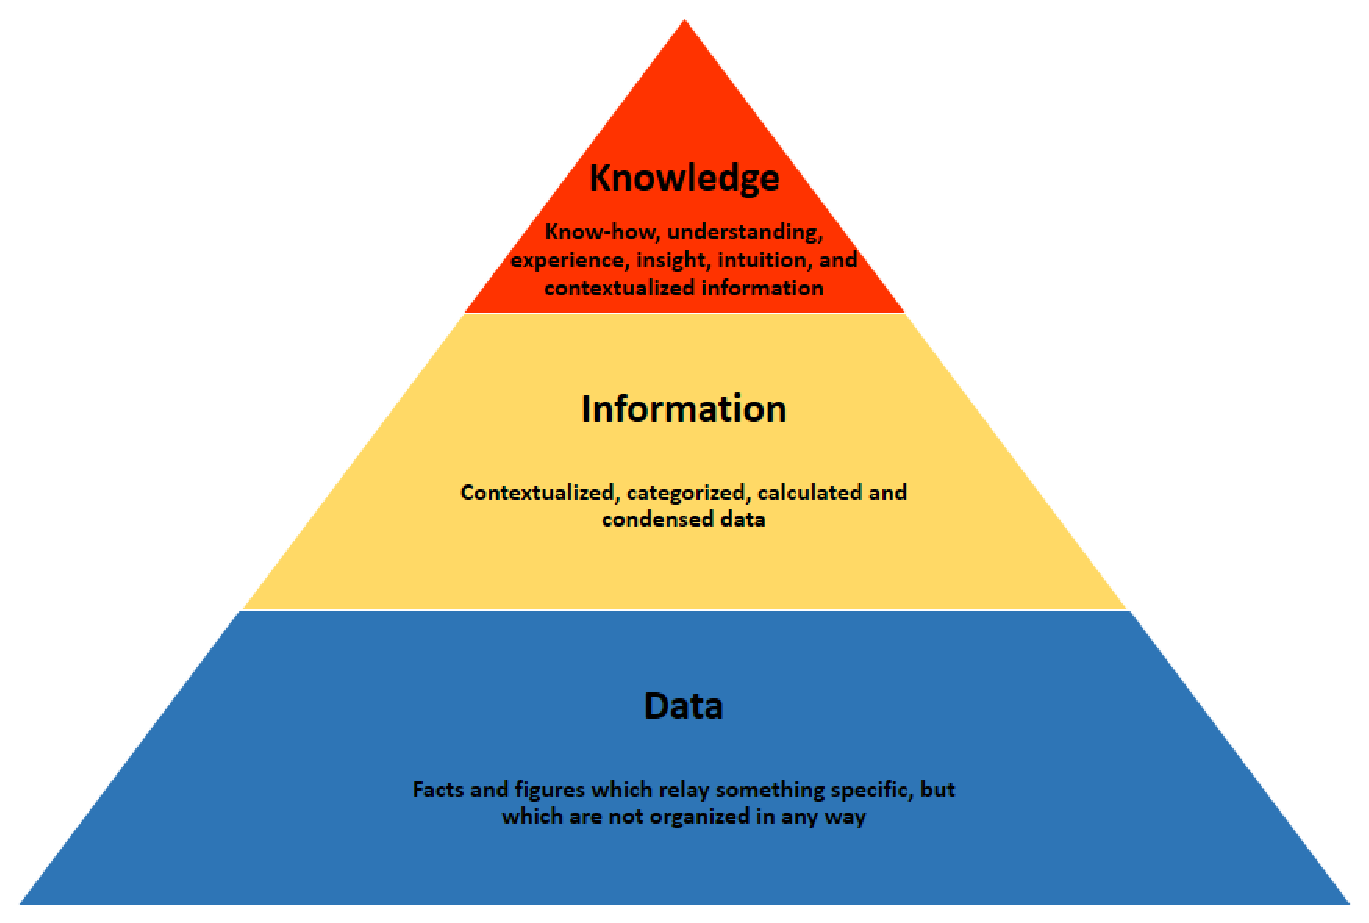
\includegraphics[width=\textwidth,height=\textheight,keepaspectratio]{figuras/piramide}
\caption{Pirámide do coñecemento}
\label{piramide}
\end{figure}

A distinción desta ferramenta con respecto a outras similares (véxase Weka) radica en que JDataMotion interpreta a temporalidade de cada instancia. Hoxe en día, case toda a información que manexamos contén polo menos un campo temporal. Na maior parte dos casos, este campo será a data na que foi tomada unha medición, ou incluso a data de inserción da mesma nunha base de datos. Estes campos non adoitan aportar por si mesmos moita información. Sen embargo, en combinación cos valores doutro campo, amosan tendencias, evolucións ou incluso indicios de que a propia variable temporal inflúe dalgún xeito nos valores.

Por unha parte, JDataMotion é unha aplicación que soluciona necesidades de información reais, e que pode ser de utilidade para calquera profesional dentro do seu campo. Esta abstracción do perfil de usuario que manexamos condicionou a toma de distintas medidas, tanto a nivel de deseño coma a nivel de implementación.

\begin{itemize}
\item A aplicación ten que empregar unha interface de usuario pouco cargada. A división en 3 menús con compoñentes mínimos non só simplificará a interface e polo tanto a experiencia do usuario, se non que ademais permitirá que se dispoña de máis espacio para amosar os datos, que son a base e motivación desta aplicación.
\item Daráselle soporte a distintos tipos de datos reais: numéricos, nominais, Strings ou datas. Entre os 4 tipos conséguese almacenar calquera valor susceptible de estar aloxado nunha base de datos, sen importar a natureza dos datos que contén, se ben os numéricos e nominais son os de maior interese para JDataMotion.
\item A aplicación intentará inferir a maior información posible do arquivo do que parte, por exemplo os tipos dos atributos en función dos seus valores. Isto repercute nun alixeiramento da fase de preprocesamento que tería que realizar o usuario manualmente. O obxectivo real do JDataMotion é visualizar datos, non manipulalos.
\item O deseño gráfico da aplicación debe gardar similitudes con outras aplicacións de escritorio similares. Elementos como as barras de menú, os botóns, menús contextuais, cadros de diálogo, etc. son característicos de moitas outras aplicacións coas que estamos familiarizados. A experiencia previa neste tipo de entornas xogará a favor da usabilidade de JDataMotion.
\item Os procesos custosos en termos de latencia serán atenuados por parte da interface gráfica, por medio dos métodos que xa vimos (barra de progreso, visualizacións da información a medida que se vai procesando, etc.).
\end{itemize}

Nun ámbito máis amplo, temos JDataMotion como proxecto, no que eu participei en calidade de xefe de proxecto, pero tamén de analista, deseñador, deseñador, controlador de calidade, etc. ao longo  das distintas fases. O proxecto comezou oficialmente coa reunión co cliente para capturar requisitos, pero o seu ciclo de vida está lonxe de acabar coa entrega do sistema e a documentación. Neste documento, de feito, pretendemos plasmar e xustificar os pasos que demos para chegar ata aquí, facilitando a formación de usuarios e futuros desenvolvedores que vaian empregar e/ou mellorar JDataMotion.

Durante o desenvolvemento que se expuxo ata agora os requisitos sufriron algunhas modificacións, ampliáronse e tamén se restrinxiron. Pese a que agora todos están completados de acordo aos tests de proba aos que foron sometidos, o proxecto está aberto a seguir engadindo ou ampliando requisitos á súa especificación. De feito, a publicación da interface de filtros xa leva implícita unha futura demanda de novos requisitos, coma por exemplo, a implementación de novos tipos de parámetros para estes, que se adapten ás necesidades dos desenvolvedores.

Outros puntos do proxecto nos que se prantexa unha mellora ou revisión son: 

\begin{itemize}
\item Volver a prantexarse a funcionalidade de difuminar puntos, mencionada no RF23. Crear un novo Dataset cunha estrutura máis permisiva pode ser un bo punto de partida.
\item Traballar en reducir máis latencia da aplicación, sobre todo no refresco do menú de Visualización. Unha suxerencia para axilizar a visualización de certo número de diagramas ao mesmo tempo, sería que estes se cargasen dinamicamente ao desprazar o scroll do menú cara a eles, en vez de todos á vez ao principio.
\item Traballar en reducir máis latencia da aplicación, sobre todo no refresco do menú de Visualización. Unha suxerencia para axilizar a visualización de certo número de diagramas ao mesmo tempo, sería que estes se cargasen dinamicamente ao desprazar o scroll do menú cara a eles, en vez de todos á vez ao principio.
\item Desenvolver uns mecanismos que fagan posible a migración de sesións, xa que se modificamos a aplicación, as sesións previas devolverán un erro de integridade.
\item Desenvolver un asistente para realizar algunhas tarefas e/ou incluír menús de axuda.
\end{itemize}

A pesar de que a metodoloxía de traballo (Scrum) foi adoptada pola miña inexperiencia neste tipo de proxectos, si que resulta moi recomendable que JDataMotion continúe adoptando algún tipo de metodoloxía áxil, e que faga partícipe ao cliente do seu desenvolvemento (sobre todo mediante probas heurísticas coa súa colaboración), para manter o proxecto á altura das expectativas que este teña.

Valorando o resultado final, pensamos que, en conxunto, as ferramentas e tecnoloxías polas que nos decantamos na fase de análise conseguiron xustificar a súa elección.

\begin{itemize}
\item Weka propuxo un conxunto de procesos eficaz para almacenar, xestionar e recuperar todos os datos do Modelo.
\item JFreeChart tiña unhas clases e métodos óptimos para xestionar os diagramas de dispersión. Algunhas clases foron sobrescritas para adecualas ao noso proxecto.
\item JUnit,  en combinación cos métodos e clases de Weka, permitiu afianzar os pasos completados, xa que podíamos comprobar que cada novo sprint completado non alteraba o correcto funcionamento dos requisitos funcionais de sprints anteriores.
\item Lumzy axudounos a descubrir cal era a interface gráfica que queríamos representar, e a crear mockups para interactuar minimamente con ela.
\item NetBeans simplificou o deseño da interface gráfica, de xeito que resultou moi áxil transportar os bocexos dos menús á ventá de JDataMotion.
\end{itemize}
